\documentclass[border=5pt]{standalone}
\usepackage{tikz}
\usepackage{xcolor}

\definecolor{danger}{RGB}{220,53,69}
\definecolor{warning}{RGB}{255,193,7}
\definecolor{secondary}{RGB}{108,117,125}
\definecolor{success}{RGB}{40,167,69}
\definecolor{primary}{RGB}{0,123,255}

\begin{document}
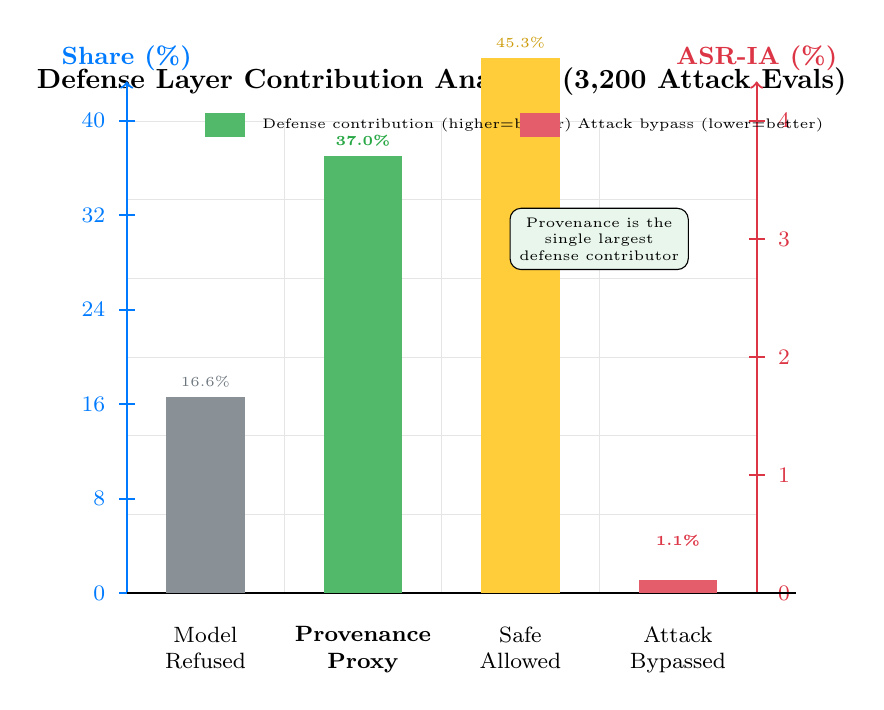
\begin{tikzpicture}[scale=1]
  % Title
  \node[font=\bfseries] at (4, 6.5) {Defense Layer Contribution Analysis (3{,}200 Attack Evals)};
  
  % Background grid
  \draw[gray!20, very thin] (0,0) grid[xstep=2, ystep=1] (8,6);
  
  % Y-axes
  % Left Y-axis (Share %)
  \draw[thick, ->, primary] (0,0) -- (0,6.5) node[above, font=\small\bfseries, primary] {Share (\%)};
  \foreach \y/\label in {0/0, 1.2/8, 2.4/16, 3.6/24, 4.8/32, 6/40} {
    \draw[thick, primary] (-0.1,\y) -- (0.1,\y);
    \node[left, font=\footnotesize, primary] at (-0.15,\y) {\label};
  }
  
  % Right Y-axis (ASR %)
  \draw[thick, ->, danger] (8,0) -- (8,6.5) node[above, font=\small\bfseries, danger] {ASR-IA (\%)};
  \foreach \y/\label in {0/0, 1.5/1, 3/2, 4.5/3, 6/4} {
    \draw[thick, danger] (7.9,\y) -- (8.1,\y);
    \node[right, font=\footnotesize, danger] at (8.15,\y) {\label};
  }
  
  % X-axis
  \draw[thick] (0,0) -- (8.5,0);
  
  % Bar positions
  \def\barwidth{0.5}
  
  % Model Refused: 16.6% -> 16.6/40*6 = 2.49
  \fill[secondary!80] (1-\barwidth, 0) rectangle (1+\barwidth, 2.49);
  \node[below, font=\footnotesize, align=center] at (1, -0.3) {Model\\Refused};
  \node[above, font=\tiny, secondary] at (1, 2.49) {16.6\%};
  
  % Provenance Proxy: 37.0% -> 37.0/40*6 = 5.55
  \fill[success!80] (3-\barwidth, 0) rectangle (3+\barwidth, 5.55);
  \node[below, font=\footnotesize\bfseries, align=center] at (3, -0.3) {\textbf{Provenance}\\Proxy};
  \node[above, font=\tiny\bfseries, success] at (3, 5.55) {\textbf{37.0\%}};
  
  % Safe Allowed: 45.3% -> 45.3/40*6 = 6.80
  \fill[warning!80] (5-\barwidth, 0) rectangle (5+\barwidth, 6.80);
  \node[below, font=\footnotesize, align=center] at (5, -0.3) {Safe\\Allowed};
  \node[above, font=\tiny, warning!80!black] at (5, 6.80) {45.3\%};
  
  % Attack Bypassed: 1.1% -> 1.1/40*6 = 0.17
  \fill[danger!80] (7-\barwidth, 0) rectangle (7+\barwidth, 0.17);
  \node[below, font=\footnotesize, align=center] at (7, -0.3) {Attack\\Bypassed};
  \node[above, font=\tiny\bfseries, danger] at (7, 0.47) {1.1\%};
  
  % Annotation
  \node[draw, rounded corners, fill=success!10, font=\tiny, align=center] at (6, 4.5) {Provenance is the\\single largest\\defense contributor};
  
  % Legend
  \fill[success!80] (1, 5.8) rectangle (1.5, 6.1);
  \node[right, font=\tiny] at (1.6, 5.95) {Defense contribution (higher=better)};
  \fill[danger!80] (5, 5.8) rectangle (5.5, 6.1);
  \node[right, font=\tiny] at (5.6, 5.95) {Attack bypass (lower=better)};
  
\end{tikzpicture}
\end{document}
